\makeheading{Week 4}{\daterange{2022-01-24}{2022-01-28}}%chktex 8
\section{Modeling of Propensity Scores}
\subsubsection*{Estimation of Propensity Scores}
\begin{itemize}
      \item In observational studies, $ \ps{x} $ is unknown and must be
            estimated.
      \item Logistic regression is the most common approach:
            \[ \logit[\big]{\ps{x}}=x^\top \beta. \]
            \begin{itemize}
                  \item For a subject with covariates $ x $, $ \estps{x}=\expit{x^\top \hat{\beta}} $.
                  \item The goal of fitting a propensity score model is not interpretation (overfitting is okay).
            \end{itemize}
\end{itemize}
Variable selection in PS model:
\begin{center}
      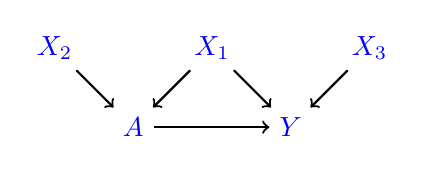
\begin{tikzpicture}[thick]
            \node (X2) at (0,0) {\textcolor{Blue}{$ X_2 $}};
            \node (X1) at (2,0) {\textcolor{Blue}{$ X_1 $}};
            \node (X3) at (4,0) {\textcolor{Blue}{$ X_3 $}};
            \node (A) at (1,-1) {\textcolor{Blue}{$ A   $}};
            \node (Y) at (3,-1) {\textcolor{Blue}{$ Y   $}};
            \draw[->] (X2) to (A);
            \draw[->] (X1) to (A);
            \draw[->] (X1) to (Y);
            \draw[->] (A) to (Y);
            \draw[->] (X3) to (Y);
      \end{tikzpicture}
\end{center}
\begin{itemize}
      \item $ X_1 $: real confounder.
      \item $ X_2 $: marginally related to the treatment.
      \item $ X_3 $: marginally related to the outcome.
      \item We should include $ X_1 $ and $ X_3 $ into the propensity score model.
\end{itemize}
\subsection*{Estimation of Propensity Scores}
Remember when we estimate propensity scores, we model $A$
(assuming binary) as a function of $X$. Therefore, we may employ
non-parametric classification methods to estimate propensity scores:
\begin{itemize}
      \item Classification and regression trees.
      \item Random forest.
      \item \textcolor{Blue}{Generalized boosted model}.
      \item Support vector machine.
      \item $K$ nearest neighbours.
\end{itemize}
\chapter{Propensity Score-Based Methods}
PS analysis is a two-step procedure:
\begin{enumerate}[1.]
      \item Estimate propensity scores $ \estps{X_i} $ for $ i=1,\ldots,n $ using data $ (A_i,X_i) $, $ i=1,\ldots,n $.
      \item Using $ \estps{X_i} $, $ i=1,\ldots,n $ to adjust the original sample and estimate causal effects:
            \begin{itemize}
                  \item Matching.
                  \item Stratification.
                  \item Inverse Probability Weighting (IPW).
                  \item Double-Robust Estimation.
            \end{itemize}
\end{enumerate}
\section{Method 1: Matching}
Basic idea: Consider matching strata, $ S_1,\ldots,S_K $
\[ \E{Y^1-Y^0}=\sum_{k=1}^{K}\E{Y^1-Y^0\given X\in S_k}\Prob{X\in S_k}, \]
where for all $ X\in S_k $, we have balance.
\begin{itemize}
      \item $ \E{Y^1-Y^0\given X\in S_k} $ may be estimated as in a randomized study by using data in $ S_k $.
      \item $ \Prob{X\in S_k}\approx \frac{\text{number of subjects in $S_k$}}{n} $.
      \item Problem: if size of $X$ is moderate or high-dimensional, it is
            hard to define the strata (curse of dimensionality).
      \item Solution: use the same stratified estimation strategy as
            before, but use $ \ps{X} $ instead of $X$ to stratify.
            \[ \E{Y^1-Y^0}=\sum_{k=1}^{K}\E[\big]{Y^1-Y^0\given \ps{X}\in S_k}\Prob[\big]{\ps{X}\in S_k}. \]
      \item Lots of different matching algorithms available
      \item One example: 1 to 1 nearest available matching on estimated
            propensity scores:
            \begin{enumerate}[1.]
                  \item Randomly order the treated and untreated (control) subjects.
                  \item Select the first treated subject and find the control subject with
                        the closest propensity score.
                  \item Both subjects are then removed from the pool and then repeat
                        step 2 until all the treated subjects are matched.
                  \item Fit an outcome model using the matched dataset.
            \end{enumerate}
\end{itemize}
\subsection*{A Toy Example}
\begin{Example}{}
      \begin{center}
            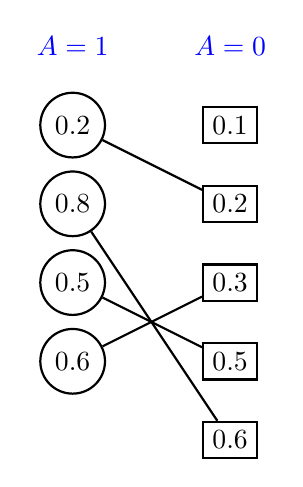
\begin{tikzpicture}[thick]
                  \node (A1) at (0,4) {\textcolor{Blue}{$A=1$}};
                  \node[circle,draw=black] (A102) at (0,3) {0.2};
                  \node[circle,draw=black] (A108) at (0,2) {0.8};
                  \node[circle,draw=black] (A105) at (0,1) {0.5};
                  \node[circle,draw=black] (A106) at (0,0) {0.6};

                  \node (A0) at (2, 4) {\textcolor{Blue}{$A=0$}};
                  \node[rectangle,draw=black] (A001) at (2,3) {0.1};
                  \node[rectangle,draw=black] (A002) at (2,2) {0.2};
                  \node[rectangle,draw=black] (A003) at (2,1) {0.3};
                  \node[rectangle,draw=black] (A005) at (2,0) {0.5};
                  \node[rectangle,draw=black] (A006) at (2,-1) {0.6};

                  \draw[-] (A102) to (A002);
                  \draw[-] (A108) to (A006);
                  \draw[-] (A105) to (A005);
                  \draw[-] (A106) to (A003);
            \end{tikzpicture}
      \end{center}
      Once the matched dataset is formed, we have
      \[ \widehat{\ACE}=\bar{Y}^{A=1,\text{matched}}-\bar{Y}^{A=0,\text{matched}}. \]
\end{Example}
Different variations of matching algorithm:
\begin{itemize}
      \item $1$ to $1$ versus $1$ to $M$ matching ($M=3$ is a common choice).
      \item \textbf{With replacement} versus \textbf{without replacement} matching.
      \item \textbf{Matching without calipers} versus \textbf{matching within calipers}
            (only two closest subjects whose propensity score difference is
            within a prespecified caliper, say, $0.2$, will be matched).
      \item Other variations.
      \item Advantage: matching based on propensity scores is far simpler
            than matching on even a modest number of risk factors
            simultaneously.
      \item Disadvantage: obtaining valid standard error of the causal
            estimator is challenging. In R, use \texttt{Matching} package.
\end{itemize}
\section{Method 2: Stratification}
Basic idea: create only a few strata; in each stratum,
individuals have similar, but not identical, values of $ \estps{X} $.
\begin{Regular}{Algorithm for Stratification}
      \begin{enumerate}[1.]
            \item Divide the subjects into $ K $ (usually $ K=5 $) strata on the basis of the quantiles
                  of $ \estps{X_i} $, $ i=1,\ldots,n $.
            \item The causal effect is estimated within each stratum as in a
                  randomized study:
                  For the $ j\textsuperscript{th} $ stratum, defined as $ S_j $:
                  \[ \widehat{\ACE}^{(j)}=\frac{\sum_{i\in S_j}Y_i A_i}{\sum_{i\in S_j}A_i}-\frac{\sum_{i\in S_j}Y_i(1-A_i)}{\sum_{i\in S_j}(1-A_i)}, \]
                  and
                  \[ \widehat{\ACE}=\frac{1}{K}\sum_{j=1}^{K}\widehat{\ACE}^{(j)}. \]
      \end{enumerate}
\end{Regular}
\begin{itemize}
      \item Advantage: Simpler than matching algorithms.
      \item Disadvantage:
            \begin{itemize}
                  \item It is possible to have no treated/untreated subjects in a
                        particular stratum.
                  \item There is no good way to obtain valid standard error of $ \widehat{\ACE} $.
            \end{itemize}
\end{itemize}
\section{Method 3: Inverse Probability Weighting}
\begin{Result}{}
      \[ \E*{\frac{AY}{\ps{X}}}=\E{Y^1}\quad\text{and}\quad \E*{\frac{(1-A)Y}{1-\ps{X}}}=\E{Y^0}. \]
      \tcblower{}
      \textbf{Proof}: Lunceford \& Davidian (2004).
      \begin{align*}
            \E*{\frac{AY}{\ps{X}}}
             & =\E*{\E*{\frac{AY}{\ps{X}}\given Y^1,X}}                                       \\
             & =\E*{\E*{\frac{AY^1}{\ps{X}}\given Y^1,X}} &  & \text{since $AY^1+(1-A)Y^0=Y$} \\
             & =\E*{\frac{Y^1}{\ps{X}}\E*{A\given Y^1,X}}                                     \\
             & =\E*{\frac{Y^1}{\ps{X}}\E{A\given X}}      &  & \text{SITA}                    \\
             & =\E*{\frac{Y^1}{\ps{X}}\ps{X}}                                                 \\
             & =\E{Y^1}.
      \end{align*}
      Similarly,
      \begin{align*}
            \E*{\frac{(1-A)Y}{1-\ps{X}}}
             & =\E*{\E*{\frac{(1-A)Y}{1-\ps{X}}\given Y^0,X}} \\
             & \vdotswithin{=}                                \\
             & =\E{Y^0}.
      \end{align*}
      We used SITA\@: $ (Y^1,Y^0)\indep (A\mid X) $, however we only need WITA\@: $ Y^1\indep (A\mid X) $ and $ Y^0\indep(A\mid X) $.
\end{Result}
\begin{itemize}
      \item Weighting scheme:
            \begin{itemize}
                  \item For those in the treatment group ($ A_i=1 $), assign a weight of $ w_i=1/\estps{X_i} $.
                  \item For those in the control group ($ A_i=0 $), assign a weight of $ w_i=1/(1-\estps{X_i}) $.
            \end{itemize}
      \item By weighting, each subject is replicated $ w_i $ times. IPW creates
            a pseudo-population in which $ A $ and $ X $ are not associated (no confounding).
\end{itemize}
\begin{Example}{Example: IPW Weighting}
      \begin{itemize}
            \item Before weighting:
                  \begin{center}
                        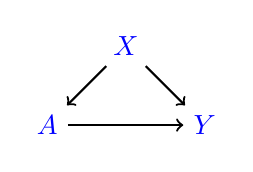
\begin{tikzpicture}[thick]
                              \node (X) at (0,1) {\textcolor{Blue}{$ X $}};
                              \node (A) at (-1,0) {\textcolor{Blue}{$ A $}};
                              \node (Y) at (1,0) {\textcolor{Blue}{$ Y $}};
                              \draw[->] (X) to (A);
                              \draw[->] (X) to (Y);
                              \draw[->] (A) to (Y);
                        \end{tikzpicture}
                  \end{center}
            \item After weighting:
                  \begin{center}
                        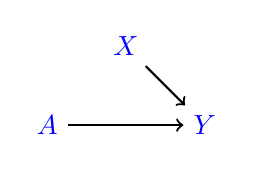
\begin{tikzpicture}[thick]
                              \node (X) at (0,1) {\textcolor{Blue}{$ X $}};
                              \node (A) at (-1,0) {\textcolor{Blue}{$ A $}};
                              \node (Y) at (1,0) {\textcolor{Blue}{$ Y $}};
                              \draw[->] (X) to (Y);
                              \draw[->] (A) to (Y);
                        \end{tikzpicture}
                  \end{center}
      \end{itemize}
      \tcblower{}
      \textcolor{Blue}{$ X $ and $ A $ are no longer confounded}.
\end{Example}
\begin{Regular}{}
      \begin{itemize}
            \item To estimate $ \E{Y^1} $, we take the \textcolor{Blue}{weighted} average of the observed $ Y $ in the treatment group, that is,
                  \[ \frac{1}{n}\sum_{i=1}^{n}\frac{A_i Y_i}{\estps{X_i}}. \]
            \item To estimate $ \E{Y^0} $, we take the \textcolor{Blue}{weighted} average of the observed $ Y $ in the control group, that is,
                  \[ \frac{1}{n}\sum_{i=1}^{n}\frac{(1-A_i)Y_i}{1-\estps{X_i}}. \]
            \item The consistent (asymptotically unbiased) estimator for ACE is:
                  \[ \hat{\tau}_{\IPW_1}= \frac{1}{n}\sum_{i=1}^{n}\frac{A_i Y_i}{\estps{X_i}}-\frac{1}{n}\sum_{i=1}^{n}\frac{(1-A_i)Y_i}{1-\estps{X_i}}. \]
            \item A more efficient estimator for ACE is:
                  \[ \hat{\tau}_{\IPW_2}=
                        \biggl(\sum_{i=1}^{n}\frac{A_i}{\estps{X_i}}\biggr)^{\!-1}
                        \sum_{i=1}^{n}\frac{A_i Y_i}{\estps{X_i}}-
                        \biggl(\sum_{i=1}^{n}\frac{1-A_i}{1-\estps{X_i}}\biggr)^{\!-1}
                        \sum_{i=1}^{n}\frac{(1-A_i)Y_i}{1-\estps{X_i}}. \]
      \end{itemize}
\end{Regular}
\begin{itemize}
      \item Properties (such as standard error) of IPW estimators should
            reflect the fact that $ \ps{X_i} $'s are estimated.
            \begin{itemize}
                  \item In R, use \texttt{survey} or \texttt{geepack} packages to get standard errors of $ \hat{\tau} $.
                  \item Bootstrap approach: A random re-sampling approach to
                        measure the accuracy of a sample estimator.
            \end{itemize}
\end{itemize}
\begin{Regular}{Bootstrap Approach for IPW}
      \begin{itemize}
            \item Sample $ b=1,\ldots,B $ (say $ B=500 $) datasets of size $ n $ \textbf{with replacement}
                  from the original data.
            \item For each bootstrapped sample, estimate $ \hat{\tau}_{\IPW_1}^{(b)} $ and $ \hat{\tau}_{\IPW_2}^{(b)} $, $ b=1,\ldots,B $.
            \item Obtain
                  \[ \estVar{\hat{\tau}_{\IPW_1}}=\frac{1}{B-1}\sum_{b=1}^{B}(\hat{\tau}_{\IPW_1}^{(b)}-\bar{\hat{\tau}}_{\IPW_1})^2, \]
                  where $ \bar{\hat{\tau}}_{\IPW_1}=\frac{1}{B}\sum_{b=1}^{B}\hat{\tau}_{\IPW_1}^{(b)} $.
            \item The same procedure applies to $ \estVar{\hat{\tau}_{\IPW_2}} $.
      \end{itemize}
\end{Regular}
\section{Method 4: Double-Robust Estimation}
\begin{itemize}
      \item Problem: If the propensity score model is incorrect, Matching,
            Stratification and IPW estimators will be biased.
      \item Solution: Combine IPW with the regression modelling
            approach to protect against model misspecification.
\end{itemize}
\begin{Regular}{}
      \begin{itemize}
            \item ``Double-robust'' means $ \hat{\tau}_{\DR} $ is consistent for ACE, if one of the following is true:
                  \begin{itemize}
                        \item The model for the propensity score, $ \ps{X,\beta} $, is correctly specified:
                              \[ \logit[\big]{\ps{X,\beta}}=X^\top \beta. \]
                        \item The models for the outcome regression, $ m_a(X;\gamma_a) $, $ a=0,1 $, are correctly specified:
                              \begin{align*}
                                    m_1(X;\gamma_1) & =\E{Y\given X,A=1}=X^\top \gamma_1. \\
                                    m_0(X;\gamma_0) & =\E{Y\given X,A=0}=X^\top \gamma_0.
                              \end{align*}
                  \end{itemize}
            \item The consistency of the estimator does not require both sets of
                  models to be correct.
            \item The DR estimator:
                  \begin{align*}
                        \hat{\tau}_{\DR}
                         & =\frac{1}{n}\sum_{i=1}^{n}\frac{A_i Y_i-[A_i-\estps{X_i}]\hat{m}_1(X_i)}{\estps{X_i}}                     \\
                         & \phantom{{}={}}-\frac{1}{n}\sum_{i=1}^{n}\frac{(1-A_i)Y_i+[A_i-\estps{X_i}]\hat{m}_0(X_i)}{1-\estps{X_i}} \\
                         & =\hat{\tau}_{1,\DR}-\hat{\tau}_{0,\DR},
                  \end{align*}
                  where $ \hat{\tau}_{1,\DR} $ estimates $ \E{Y^1} $ and $ \hat{\tau}_{0,\DR} $ estimates $ \E{Y^0} $.
      \end{itemize}
      \tcblower{}
      \underline{Remark}: The above estimator is also called augmented estimator
      since it can be viewed as taking the inverse weighted
      estimator and ``augmenting'' it by a second term.
\end{Regular}
\begin{Regular}{Implementation of Double-Robust Estimation}
      \begin{enumerate}[1.]
            \item Fit logistic regression model for the propensity score
                  \[ \logit[\big]{\Prob{A_i=1\given X_i=x_i}}=x_i^\top \beta,\qquad \widehat{\textsf{ps}}_i=\expit{x_i^\top \hat{\beta}}. \]
            \item Fit regression model for the outcome using data from the
                  treatment group only, predict for all subjects
                  \[ \E{Y_i\given X_i=x_i,A_i=1}=x_i^\top \gamma_1,\qquad \hat{m}_1(x_i)=x_i^\top\hat{\gamma}_1. \]
            \item Fit a regression model for the outcome (same form as above)
                  using data from the control group only, predict for all subjects
                  \[ \E{Y_i\given X_i=x_i,A_i=0}=x_i^\top \gamma_0,\qquad \hat{m}_0(x_i)=x_i^\top\hat{\gamma}_0. \]
            \item Plug in predicted values into the expression for $ \hat{\tau}_{\DR} $.
      \end{enumerate}
\end{Regular}
\begin{itemize}
      \item Properties (such as standard error) of the DR estimator should
            reflect the fact that $ \ps{X_i} $'s are estimated.
      \item A formula for the theoretical standard error
            \[ \estVar{\hat{\tau}_{\DR}}=\frac{1}{n^2}\sum_{i=1}^{n}\hat{I}_i^2, \]
            where
            \begin{align*}
                  \hat{I}_i
                   & =\frac{A_i Y_i-[A_i-\estps{X_i}]\hat{m}_1(X_i)}{\estps{X_i}}                     \\
                   & \phantom{{}={}}-\frac{(1-A_i)Y_i+[A_i-\estps{X_i}]\hat{m}_0(X_i)}{1-\estps{X_i}} \\
                   & \phantom{{}={}}-\hat{\tau}_{\DR}.
            \end{align*}
            Note: The formula only works well if both the propensity score
            and outcome regression models are correctly specified.
\end{itemize}
\begin{Regular}{Bootstrap Approach for Double-Robust Estimation}
      \begin{itemize}
            \item Sample $ b=1,\ldots,B $ (say $ B=500 $) datasets of size $ n $ \textbf{with replacement}
                  from the original data.
            \item For each bootstrapped sample, estimate $ \hat{\tau}_{\DR}^{(b)} $, $ b=1,\ldots,B $.
            \item Obtain
                  \[ \estVar{\hat{\tau}_{\DR}}=\frac{1}{B-1}\sum_{b=1}^{B}(\hat{\tau}_{\DR}^{(b)}-\bar{\hat{\tau}}_{\DR})^2, \]
                  where $ \bar{\hat{\tau}}_{\DR}=\frac{1}{B}\sum_{b=1}^{B}\hat{\tau}_{\DR}^{(b)} $.
      \end{itemize}
\end{Regular}
\section{Case Study I: Propensity Score Analysis}
\textbf{Propensity Score Methods}:
\begin{itemize}
      \item Matching.
      \item Stratification.
      \item Inverse Probability Weighting.
      \item Double-Robust Estimation.
\end{itemize}
